% =====================================================================
%  Capitolo 2 — Sistemi di intonazione
%  STATO: scheletro delle sezioni dall'Indice; testo DA TRASCRIVERE.
% =====================================================================
\chapter{Sistemi di intonazione}

Scopo della seconda parte di questa trattazione è descrivere la funzione
strutturale degli intervalli nella definizione di alcuni sistemi di
intonazione. Pertanto esula dalle nostre intenzioni procedere a qualsiasi
analisi di tipo comparativo o estetico rispetto ai sistemi presi in esame.

Un sistema di intonazione consiste nella proiezione di un numero finito di
intervalli nell'ambito del rapporto $2/1$ o ottava.

Gli intervalli che formano un sistema di intonazione vengono derivati da una
delle tre procedure seguenti: \emph{serie delle quinte}, \emph{numeri naturali}
e \emph{radicali}.

Nel primo caso essi vengono ricavati moltiplicando o dividendo l'intervallo
base $3/2$ (quinta) per se stesso tante volte quante sono le altezze che si
vuole formino il sistema. Chiaramente, essendo i risultati di ciascuna
operazione sempre diversi, l'intero sistema, oltre a dividere l'ottava in parti
ineguali, può essere formato teoricamente da una infinita serie di altezze.

Nella seconda procedura invece gli intervalli vengono ricavati moltiplicando o
dividendo i rapporti risultanti dalla serie dei numeri naturali. Anche in
questo caso l'ottava risulterà divisa in parti ineguali e il sistema può essere
formato da una infinita serie di altezze.

In ultimo, gli intervalli vengono ricavati applicando le radici del fattore
primo 2 (ottava). È questo il caso, tra gli altri, del temperamento equabile
dove i 12 semitoni vengono appunto derivati da $\sqrt[12]{2}$. Dissimilmente
dalle altre procedure il numero delle parti in cui si trova ad essere divisa
l'ottava, oltre che essere equidistante, è strutturalmente finito in quanto
deciso in partenza.

Il numero e la complessità degli intervalli che formano un sistema di
intonazione può mutare a seconda del tipo di pratica musicale che, come si sa,
quando è monodica utilizza un sistema di intervalli complesso poiché
l'espressività musicale si impernia essenzialmente sulla singola melodia,
mentre quando è polifonica gli intervalli sono più semplici data la necessità
di dover sovrapporre più disegni melodici contemporaneamente.

Particolarità di un sistema di intonazione è che gli intervalli che lo
compongono non perdono la loro identità qualora trasposti nelle diverse ottave.
In altre parole, se prendiamo come esempio l'intervallo di quinta $384:256$,
esso rimane lo stesso anche nel rapporto frequenziale $768:512$ oppure in quello
$48:32$. Esiste una distinzione tra sistema e scala musicale in quanto
quest'ultima è costituita dall'arrangiamento in successione, nello spazio di
un'ottava, di tutti, o parte, gli intervalli propri di un sistema. Vale a dire
che da uno stesso sistema di intervalli si possono ricavare più scale come, ad
esempio, da quello del temperamento equabile la scala maggiore, minore melodica
ascendente e discendente, minore armonica, per toni interi, pentatonica e molte
altre.

Come abbiamo visto i sistemi di intonazione differiscono sostanzialmente per la
natura degli intervalli che li costituiscono. Si hanno quindi sistemi detti
\emph{naturali} quando gli intervalli sono puri acusticamente parlando, quando
derivano direttamente dai rapporti matematici ricavabili dalle successive
divisioni della corda. I principali sistemi che appartengono a questa categoria
sono quello pitagorico e quello naturale (\emph{Just Intonation}).
Differentemente un sistema è \emph{temperato} quando gli intervalli che lo
formano deviano da quelli acusticamente corretti. A questa seconda categoria
appartengono numerosi temperamenti.

A questo proposito vale la pena ricordare che nel corso del diciassettesimo
secolo erano in uso simultaneamente almeno una ventina di temperamenti diversi,
tanto che teorici musicali come Giovanni Maria Artusi ed Ercole Bottrigari
riportano nei loro scritti che non era possibile far suonare più strumenti
insieme a causa dei sistemi di intonazione così divergenti. Tuttavia, tra i
molti temperamenti che si sono succeduti nelle diverse epoche, soprattutto due
hanno avuto una rilevanza storica: quello non equabile \emph{Sistema participato
mesotonico}, così chiamato da Bartolomeo Ramis nel trattato \emph{Musica
practica} (Bologna 1482) e conosciuto anche come sistema del tono medio
(\emph{Mean-tone}), e il ben noto temperamento equabile, la cui soluzione,
consistente appunto nella normalizzazione a 12 semitoni uguali nello spazio di
un'ottava, fu studiata da Simon Stevin e messa in pratica intorno al 1690 da
Andreas Werkmeister nella costruzione dei suoi organi.\footnote{La prima
apparizione del temperamento equabile documentata fu in Cina dove la brillante
soluzione prospettata dal principe Tsai-Yü rimane un enigma poiché la musica
cinese non richiede alcun tipo di temperamento.}

La storia dei temperamenti è intimamente connessa a quella degli strumenti
musicali e le ragioni che hanno portato ai vari metodi di intonazione sono da
ricercarsi probabilmente nella esigenza di semplificazione e operatività degli
strumenti stessi, come la disposizione dei fori nel flauto o nel clarinetto o
la lunghezza delle corde nella lira o nell'arpa, ma la storia del temperamento
equabile è legata soprattutto alla discretizzazione e standardizzazione delle
altezze negli strumenti a tastiera.

% =====================================================================
\section{Sistemi di intonazione temperati a divisione semplice e multipla}

Con l'impiego dei radicali è possibile ottenere infinite divisioni dell'ottava,
o qualsiasi altro intervallo, in parti equidistanti. Riporteremo qui alcuni
esempi di divisione. Nel primo caso l'intervallo di ottava viene diviso in 24
parti uguali (quarti di tono). Per far ciò, utilizzando la stessa procedura
impiegata per il calcolo dei 12 semitoni del temperamento equabile, si è
proceduto inizialmente al calcolo della radice ventiquattresima di due:
\[
  \sqrt[24]{2} = 1{,}029302237
\]
quindi, una volta ricavato il coefficiente $1{,}029302237$, si procede alla
moltiplicazione di questo, a partire da un valore frequenziale, ad esempio di
$100$~Hz, tante volte quanto è il numero delle suddivisioni nell'ottava.
Avremo così ottenuto un sistema di altezze strutturato nel modo
seguente:\footnote{Tutti i numeri sono stati troncati ad una cifra decimale.}

\begin{center}\small
\begin{tabular}{r l@{\qquad\qquad}r l}
 1) & 100~Hz & 13) & 141{,}4 \\
 2) & 102{,}9 & 14) & 145{,}5 \\
 3) & 105{,}9 & 15) & 149{,}8 \\
 4) & 109     & 16) & 154{,}2 \\
 5) & 112{,}2 & 17) & 158{,}7 \\
 6) & 115{,}5 & 18) & 163{,}3 \\
 7) & 118{,}9 & 19) & 168{,}1 \\
 8) & 122{,}4 & 20) & 173{,}1 \\
 9) & 125{,}9 & 21) & 178{,}1 \\
10) & 129{,}6 & 22) & 183{,}4 \\
11) & 133{,}4 & 23) & 188{,}7 \\
12) & 137{,}3 & 24) & 194{,}3 \\
    &         & 25) & 200     \\
\end{tabular}
\end{center}

Come sappiamo il radicando 2 rappresenta l'intervallo di ottava, ma se si
volesse dividere in 24 parti non più lo spazio di un'ottava ma quello di una
quinta temperata, allora bisognerà semplicemente sostituire il radicando 2 con
$1{,}498307077$ (quinta temperata) per ricavare il relativo coefficiente:
\[
  \sqrt[24]{1{,}498307077} = 1{,}016990044
\]
ed ottenere quindi un sistema di intervalli come segue:

\begin{center}\small
\begin{tabular}{r l@{\qquad\qquad}r l}
 1) & 100~Hz & 13) & 122{,}4 \\
 2) & 101{,}7 & 14) & 124{,}5 \\
 3) & 103{,}4 & 15) & 126{,}6 \\
 4) & 105{,}2 & 16) & 128{,}8 \\
 5) & 107     & 17) & 131     \\
 6) & 108{,}8 & 18) & 133{,}2 \\
 7) & 110{,}7 & 19) & 135{,}4 \\
 8) & 112{,}5 & 20) & 137{,}8 \\
 9) & 114{,}4 & 21) & 140     \\
10) & 116{,}4 & 22) & 142{,}4 \\
11) & 118{,}3 & 23) & 144{,}9 \\
12) & 120{,}3 & 24) & 147{,}3 \\
    &         & 25) & 149{,}9 \\
\end{tabular}
\end{center}

Com'è stato già detto in precedenza, un insieme di intervalli non deve essere
necessariamente considerato come scala musicale, ma piuttosto come sistema di
intervalli dal quale è possibile ricavare uno o più tipi di scale diverse.

Nell'esempio successivo lo spazio di una ottava più un semitono (nona minore)
viene diviso in 12 parti uguali. Ciò si ottiene moltiplicando per 2 il
coefficiente del semitono in modo da ottenere lo spazio desiderato.

\begin{figure}[htbp]
  \centering
  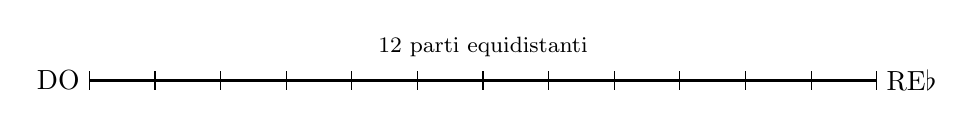
\begin{tikzpicture}[x=1cm,y=1cm]
    \draw[thick] (0,0) -- (10,0);
    \foreach \i in {0,...,12}{\draw (\i*10/12,-0.12) -- (\i*10/12,0.12);}
    \node[left] at (0,0) {DO};
    \node[right] at (10,0) {RE$\flat$};
    \node[above,font=\footnotesize] at (5,0.18) {12 parti equidistanti};
  \end{tikzpicture}
\end{figure}

\[
  \text{DO--RE}\flat = 1{,}059463094 \times 2 = 2{,}118926189
\]
(spazio di una nona minore); quindi si procede a ricavare il coefficiente:
\[
  \sqrt[12]{2{,}118926189} = 1{,}064575137\ldots
\]
Il coefficiente così ottenuto, moltiplicato 12 volte a partire da una frequenza
di $100$~Hz, darà una serie di altezze così composta:

\begin{center}\small
\begin{tabular}{r l@{\qquad\qquad}r l}
 1) & 100~Hz & 8)  & 154{,}9 \\
 2) & 106{,}4 & 9)  & 164{,}9 \\
 3) & 113{,}3 & 10) & 175{,}6 \\
 4) & 120{,}6 & 11) & 186{,}9 \\
 5) & 128{,}4 & 12) & 199     \\
 6) & 136{,}7 & 13) & 211{,}9 \\
 7) & 145{,}5 &     &         \\
\end{tabular}
\end{center}

Un'ulteriore possibilità è data dal dividere l'intervallo di ottava, o
qualsiasi altro intervallo, in modo multiplo, vale a dire prima diviso in un
numero arbitrario di parti e poi ciascuna di queste divisa ancora in un numero
arbitrario di sottoparti. Nell'esempio seguente l'ottava viene divisa in tre
parti, ognuna formata da una terza maggiore, e poi ogni terza maggiore viene a
sua volta suddivisa successivamente in 5, 6 e 7 sottoparti equidistanti.

\begin{figure}[htbp]
  \centering
  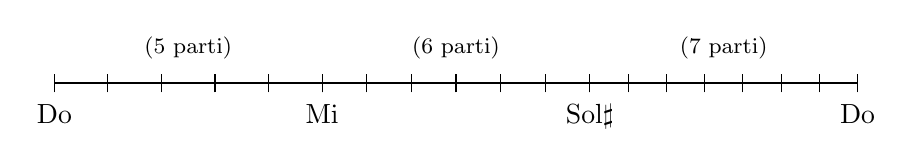
\begin{tikzpicture}[x=0.85cm,y=1cm]
    \draw[thick] (0,0) -- (12,0);
    % suddivisioni: Do-Mi 5 parti, Mi-Sol# 6 parti, Sol#-Do 7 parti
    \foreach \k in {0,...,5}{\draw (\k*4/5,-0.12) -- (\k*4/5,0.12);}
    \foreach \k in {0,...,6}{\draw (4+\k*4/6,-0.12) -- (4+\k*4/6,0.12);}
    \foreach \k in {0,...,7}{\draw (8+\k*4/7,-0.12) -- (8+\k*4/7,0.12);}
    \node[below] at (0,-0.15)  {Do};
    \node[below] at (4,-0.15)  {Mi};
    \node[below] at (8,-0.15)  {Sol$\sharp$};
    \node[below] at (12,-0.15) {Do};
    \node[above,font=\footnotesize] at (2,0.18)  {(5 parti)};
    \node[above,font=\footnotesize] at (6,0.18)  {(6 parti)};
    \node[above,font=\footnotesize] at (10,0.18) {(7 parti)};
  \end{tikzpicture}
\end{figure}

Essendo in questo caso l'ottava divisa in tre intervalli uguali (terze
maggiori), basterà trovare lo spazio di una sola terza maggiore:
\[
  \sqrt[12]{2} = 1{,}059463094^{4} = 1{,}25992105
\]
per poi procedere a trovare i tre diversi coefficienti:
\begin{align*}
  \text{Primo coefficiente}   &\quad \sqrt[5]{1{,}25992105} = 1{,}047294123 \\
  \text{Secondo coefficiente} &\quad \sqrt[6]{1{,}25992105} = 1{,}039259226 \\
  \text{Terzo coefficiente}   &\quad \sqrt[7]{1{,}25992105} = 1{,}033557783
\end{align*}
Ora, moltiplicando ciascun coefficiente per il numero delle rispettive
sottoparti nello spazio delle tre terze maggiori successive, partendo da una
frequenza di $100$~Hz, si otterrà un sistema di altezze così articolato:

\begin{center}\small
\begin{tabular}{r l@{\quad}r l@{\quad}r l}
1) & 100~Hz & 1) & 125{,}9 & 1) & 158{,}7 \\
2) & 104{,}7 & 2) & 130{,}9 & 2) & 164     \\
3) & 109{,}6 & 3) & 136     & 3) & 169{,}5 \\
4) & 114{,}8 & 4) & 141{,}4 & 4) & 175{,}2 \\
5) & 120{,}3 & 5) & 146{,}9 & 5) & 181{,}1 \\
6) & 125{,}9 & 6) & 152{,}7 & 6) & 187{,}3 \\
   &         & 7) & 158{,}7 & 7) & 193{,}5 \\
   &         &    &         & 8) & 200     \\
\end{tabular}
\end{center}

In generale, indicando con $n$, $m$ ed $l$ il numero delle sottoparti, le
altezze del sistema si ottengono con:
\[
  \sqrt[n]{\left(\sqrt[12]{2}\right)^{4}} \times
  \sqrt[m]{\left(\sqrt[12]{2}\right)^{4}} \times
  \sqrt[l]{\left(\sqrt[12]{2}\right)^{4}} \times f = \text{altezze}
\]

% =====================================================================
\section{Sistema di intonazione participato mesotonico}

Il sistema participato mesotonico è anche conosciuto come \emph{vecchio
temperamento ineguale} o \emph{nuovo temperamento}. Questo sistema, utilizzato
per oltre due secoli, riveste un ruolo preminente nella storia della musica
strumentale ed è stato per lungo tempo l'unico antagonista del temperamento
equabile. Difatti esso era in uso quasi universalmente nella pratica musicale
occidentale intorno al 1700. Fatto risalire a Gioseffo Zarlino
(\emph{Dimostrazioni harmoniche}, Venezia 1571) e allo spagnolo Francisco
Salinas (\emph{De Musica Libri VII}, Salamanca 1577), sebbene già ampiamente
spiegato nel trattato di Pietro Aron (\emph{Toscanello in musica}, Venezia
1523), pare avesse origini assai più remote (Bartolomeo Ramis e oltre). Questo
sistema, composto da terze maggiori naturali e quinte temperate, consiste nel
far combinare la terza maggiore risultante dalla serie di quattro quinte
consecutive (DO SOL RE LA MI) con la terza maggiore naturale risultante da due
ottave più una terza maggiore. Essendo l'intervallo risultante dalle quattro
quinte ($3 \times 3 \times 3 \times 3 = 81$) $81/64 = 81:64 = 404{,}8$ cents più
alto di un comma sintonico rispetto alla terza maggiore naturale
($5/4 = 386{,}3$ cents):
\[
  \frac{81}{64} \times \frac{4}{5} = \frac{324}{320} = \frac{81}{80}
\]
nel sistema participato ad un quarto di comma si è proceduto all'abbassamento
(temperamento o participazione) di ognuna delle quattro quinte successive di
$1/4$ di comma, $\sqrt[4]{5} = 1{,}49534 = 696{,}6$ cents invece di $1{,}5 = 702$
cents che caratterizza la quinta esatta, in modo tale che la quarta quinta
potesse essere di un intero comma sintonico più bassa e quindi coincidere con la
terza maggiore naturale.

Il nome di questo sistema deriva dal fatto che, in base a tale temperamento,
l'intervallo di un tono corrisponde alla media aritmetica tra il tono grande
$9/8$ e il tono piccolo $10/9$ del sistema naturale, in modo da ottenere che
l'intervallo di terza maggiore sia diviso in due toni di $193{,}2$ cents e
quindi esattamente uguali:
\[
  \frac{10}{9} \times \frac{9}{8} = \frac{5}{4} = 386{,}3~\text{cents}
\]
che diviso 2 darà appunto $193{,}2$ cents. Oppure, rispetto al sistema
pitagorico, il valore del tono medio sarà ricavato sommando i due toni $9/8$
abbassati ciascuno di mezzo comma sintonico e dividendo successivamente per 2:
\[
  \frac{9}{8} \times \frac{9}{8} = \frac{81}{64}
  \qquad
  \frac{81}{64} \times \frac{80}{81} = \frac{5}{4}
\]
La distinzione tra tono grande ($204$ cents) e tono piccolo ($182$ cents) viene
abolita dal tono medio ($193{,}2$ cents). Il semitono diatonico ($112$ cents)
diviene di $117{,}1$ cents e il semitono cromatico ($92$ cents) è di $76$ cents.

\begin{figure}[htbp]
  \centering\setlength{\tabcolsep}{4pt}
  \resizebox{\textwidth}{!}{%
  \begin{tabular}{*{13}{c}}
    Do & Do$\sharp$ & Re & Mi$\flat$ & Mi & Fa & Fa$\sharp$ & Sol & Sol$\sharp$
       & La & Si$\flat$ & Si & Do \\
    \addlinespace
    0 & 76 & 193,2 & 310,3 & 386,3 & 503,4 & 579,5 & 696,6 & 772,6 & 889,7
      & 1006,8 & 1082,9 & 1200 \\
  \end{tabular}}
\end{figure}

Questa procedura porta ad una scala che, rispetto a quella pitagorica, sarà così
configurata (v.\ schema del sistema mesotonico participato di $1/4$ di comma):

\begin{figure}[htbp]
  \centering
  \resizebox{\textwidth}{!}{%
  \begin{tabular}{l*{8}{c}}
    pitagorica: & Do & Re & Mi & Fa & Sol & La & Si & Do \\
                & 0 & 204 & 386,3 & 498 & 702 & 884 & 1088 & 1200 \\
    \addlinespace
    mesotonica: & Do & Re$^{-1/2}$ & Mi$^{-1}$ & Fa$^{+1/4}$ & Sol$^{-1/4}$
                & La$^{-3/4}$ & Si$^{-5/4}$ & Do \\
                & 0 & 193,2 & 386,2 & 503,4 & 696,6 & 889,7 & 1082,9 & 1200 \\
  \end{tabular}}
\end{figure}

e nella sua forma completa risulterà:

\begin{figure}[htbp]
  \centering\setlength{\tabcolsep}{5pt}
  \resizebox{\textwidth}{!}{%
  \begin{tabular}{*{13}{c}}
    Do & Do$\sharp^{-7/4}$ & Re$^{-1/2}$ & Mi$\flat^{+3/4}$ & Mi$^{-1}$
       & Fa$^{+1/4}$ & Fa$\sharp^{-3/2}$ & Sol$^{-1/4}$ & Sol$\sharp^{-2}$
       & La$^{-3/4}$ & Si$\flat^{+1/2}$ & Si$^{-5/4}$ & Do \\
  \end{tabular}}
\end{figure}

Da quanto detto precedentemente, l'intero sistema sarà pertanto ricavato da tre
serie di quattro quinte abbassate ciascuna di $1/4$ di comma sintonico (come
semplificazione rispetto a DO, due serie verso l'alto ed una verso il basso):

\begin{figure}[htbp]
  \centering
  \resizebox{\textwidth}{!}{%
  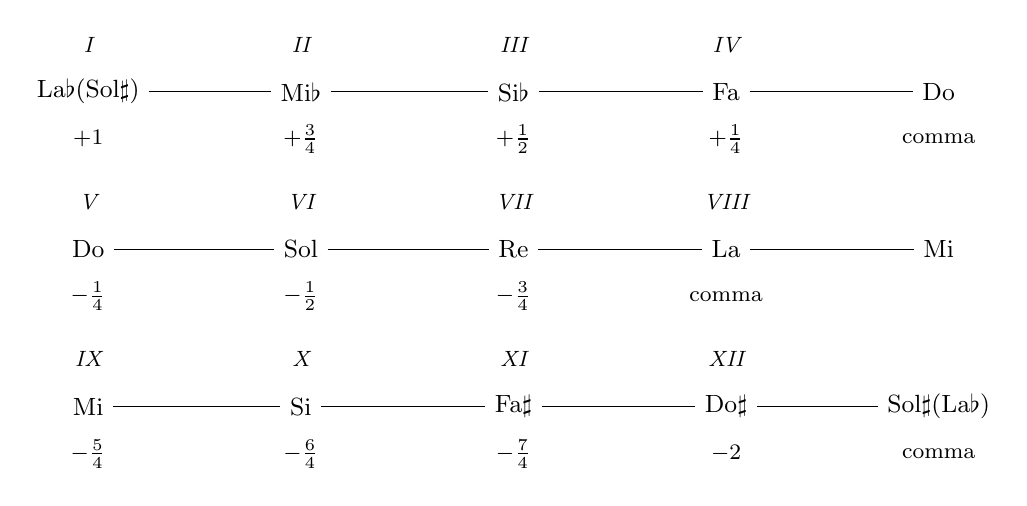
\begin{tikzpicture}[x=2.7cm,y=1cm,
      nota/.style={font=\small},
      rn/.style={font=\footnotesize\itshape},
      adj/.style={font=\footnotesize}]
    % --- serie A: verso il basso (bemolli) ---
    \foreach \x/\n/\r/\a in {%
        0/{La$\flat$(Sol$\sharp$)}/I/$+1$, 1/{Mi$\flat$}/II/$+\frac34$,
        2/{Si$\flat$}/III/$+\frac12$, 3/{Fa}/IV/$+\frac14$, 4/{Do}//comma}{
      \node[nota] (A\x) at (\x,4) {\n};
      \ifx\r\empty\else\node[rn] at (\x,4.6) {\r};\fi
      \node[adj] at (\x,3.4) {\a};
    }
    \draw (A0)--(A1)--(A2)--(A3)--(A4);
    % --- serie B: verso l'alto ---
    \foreach \x/\n/\r/\a in {%
        0/{Do}/V/$-\frac14$, 1/{Sol}/VI/$-\frac12$, 2/{Re}/VII/$-\frac34$,
        3/{La}/VIII/comma, 4/{Mi}//{}}{
      \node[nota] (B\x) at (\x,2) {\n};
      \ifx\r\empty\else\node[rn] at (\x,2.6) {\r};\fi
      \node[adj] at (\x,1.4) {\a};
    }
    \draw (B0)--(B1)--(B2)--(B3)--(B4);
    % --- serie C: verso l'alto (diesis) ---
    \foreach \x/\n/\r/\a in {%
        0/{Mi}/IX/$-\frac54$, 1/{Si}/X/$-\frac64$, 2/{Fa$\sharp$}/XI/$-\frac74$,
        3/{Do$\sharp$}/XII/$-2$, 4/{Sol$\sharp$(La$\flat$)}//comma}{
      \node[nota] (C\x) at (\x,0) {\n};
      \ifx\r\empty\else\node[rn] at (\x,0.6) {\r};\fi
      \node[adj] at (\x,-0.6) {\a};
    }
    \draw (C0)--(C1)--(C2)--(C3)--(C4);
  \end{tikzpicture}}
\end{figure}

Come risulta dallo schema, il LA$\flat$ temperato (prima nota della serie), per
effetto della somma dei $4/4$ di comma, è più alto di un intero comma sintonico
o $21{,}5$ cents rispetto al LA$\flat$ pitagorico, mentre il SOL$\sharp$ (ultima
nota della serie), per lo stesso motivo, è invece più basso di due commi o $43$
cents rispetto al SOL$\sharp$ pitagorico.

Sappiamo inoltre che, a causa del comma ditonico $531441/524288$ (vedi sistema
di intonazione pitagorico), il SOL$\sharp$ pitagorico è più alto del LA$\flat$
pitagorico (della stessa serie delle quinte pitagoriche, $12^{\text{a}}$ quinta)
di $23{,}5$ cents. Considerando quanto detto, il SOL$\sharp$ temperato finale
risulterà a questo punto $43 + 21{,}5 = 23{,}5 = 41$ cents più alto del
LA$\flat$ iniziale, temperato di circa $1/4$ di tono (differenza chiamata
\emph{Diesis}). Quindi l'intervallo di quinta SOL$\sharp$--Mi$\flat$ sarà
formato da $696{,}6$ (valore in cents della quinta temperata) $+ 41$ cents di
scarto $= 737{,}6$ cents. Questo intervallo di quinta, data la sua discordanza
rispetto alle altre, era chiamato \emph{quinte-de-loup} o \emph{quinta del
lupo}. Oltre a questa quinta si ha la presenza delle false terze Si--Mi$\flat$,
Fa$\sharp$--Si$\flat$, Do$\sharp$--Fa$\sharp$, Sol$\sharp$--Do.

Deve essere considerato anche che nella scala di Mi Maggiore dobbiamo impiegare
Mi$\flat$ al posto di Re$\sharp$ e questo conduce ancora ad un errore di $41$
cents, come pure avviene in quella di Mi$\flat$ che comporta l'introduzione di
Sol$\sharp$ al posto di La$\flat$. Tuttavia, per quanto il sistema mesotonico
risultasse soddisfacente sia melodicamente che armonicamente, a causa di tali
intervalli poteva essere impiegato soltanto in un ambito ristretto di tonalità
(da tre diesis a due bemolli). Un inconveniente del genere si poteva in parte
ovviare aumentando il numero degli intervalli nell'ottava. Vale la pena
ricordare a questo proposito come Nicola Vicentino, nel suo archicembalo a sei
tastiere, impiegava il sistema participato ordinario ottenendo così la divisione
dell'ottava in 31 parti ineguali.\footnote{Nicola Vicentino, \emph{L'antica
musica ridotta alla moderna prattica}, Roma 1555.}

Esistevano altre varietà di sistemi participati, oltre quello detto ordinario,
in cui le quinte venivano abbassate di $1/3$ o $1/5$ o $2/7$ di comma e persino
con varie combinazioni tra loro, ma il temperamento di $1/4$ di comma per quinta
risultò essere, nel suo complesso, il più soddisfacente
musicalmente.\footnote{R.~M.~H. Bosanquet, \emph{An Elementary Treatise on
Musical Intervals and Temperaments}, London 1876.}

\section{Costruzione di un sistema di intonazione non temperato}
% TODO trascrivere

\section{Sistema pitagorico}
% TODO trascrivere

\section{Tetracordo, generi e sistemi nella musica greca}
% TODO trascrivere

\subsection{Generi}
% TODO trascrivere

\subsection{Sistema perfetto}
% TODO trascrivere

\subsection{Nome delle corde della \emph{Lira} rispetto alle note nel
            collegamento di due tetracordi}
% TODO trascrivere

\subsection{Specie di ottava}
% TODO trascrivere

\section{Sistema naturale}
% TODO trascrivere

\section{Oltre il fattore 5}
% TODO trascrivere

\section{Altra possibilità di organizzazione degli intervalli derivante dai
         fattori generativi 2, 3 e 5}
% TODO trascrivere
